\label {fs-acker-intro}

There are plenty of data processing scenarios where results are most valuable at the time of data arrival, for example, IoT, news processing, financial analysis, fraud detection, and network monitoring. For such problems, one can apply a stream processing model: a processing system ingests input elements, transform them according to a logical dataflow graph consisting of data processing operators, and deliver output elements. However, regular blocking data processing operators read an entire input before producing an output and can never release a result in the case of a stream. To handle this problem, one can divide the whole unbounded, potentially infinite data stream into bounded, possibly overlapping substreams˜\cite{tucker2003exploiting}. In this case, an operator can produce an output when a corresponding substream terminates.

Distributed stream processing engines (SPEs), such as Flink~\cite{carbone2015apache}, Heron~\cite{Kulkarni:2015:THS:2723372.2742788}, or MillWheel~\cite{Akidau:2013:MFS:2536222.2536229} aim to process intensive data streams at scale. They are deployed on clusters consisting of tens or even hundreds of nodes that receive input data elements one by one, process them, and update the internal state. Within these systems, the data elements are distributed among all computational nodes in a cluster. Therefore, it is a challenging task to detect that a substream terminates system-wide. 

The following scenarios illustrate the practical importance of this problem.

\noindent {\bf Windowed aggregations}. One way to adapt a relational query to a streaming environment is to run it on a window of data elements. This way, an initial stream will be converted into a stream of query results for each window instance. This method is widely applied in online analytics~\cite{traub2018scotty} and is used for streaming SQL implementation~\cite{Begoli:2019:OSR:3299869.3314040}. The window definition, in this case, forms a substream. For example, a sliding window will define a substream for each message in the initial stream.

\noindent {\bf State pruning}. Most SPEs group state by keys that are also used for data partitioning. For example, the task is to aggregate news into stories assigning every news item a story tag. In this case, a story tag will be the key; the properties of the story that are needed for tagging procedure will be the state. The number of stories is not limited, and to prevent overflow~\cite{Tucker:2003:EPS:776752.776780}, SPE can remove state for outdated keys, e.g., for completed stories. In this case, we can consider the stream as a mixture of substreams: one per story.  

\noindent {\bf State snapshotting}. Epoch-based state snapshotting is a popular recovery technique applied in Flink~\cite{Carbone:2017:SMA:3137765.3137777}, Storm~\cite{Toshniwal:2014:STO:2588555.2595641}, Samza~\cite{Noghabi:2017:SSS:3137765.3137770}, IBM Streams~\cite{jacques2016consistent}. This method divides a stream into a sequence of data element chunks called ({\em epochs}). An SPE takes a state snapshot when a regular epoch is {\em atomically} processed. In case of failures, SPE can consistently recover the state from the snapshot~\cite{2015arXiv150608603C}. 

Each of these scenarios is a particular case of a problem of monitoring substreams emergence and termination that we call a {\em substream management problem}. A substream is a part of the stream such that all its elements satisfy some predicate. 
For example, in the case of state pruning, the predicate is {\em [a data element key equals to $K$]}, for time window aggregations, the predicate is {\em [a data element has a timestamp less than $T$]}, and for state snapshotting it is {\em [a data element belongs to the epoch $E$]}.

In this paper, we focus only on two signals: substream start and its termination. Tracking a start of a substream is a straightforward task: the first event of a substream will naturally trigger its start. On the contrary, generating a substream termination event is a challenging task, and various properties may be required by practical problems:
\begin{itemize}
    \item Deterministic windowed join\footnote{given the same sequences of input tuples, the same output tuples will be produced} requires an order of termination signals to respect the order of input elements (termination events from data producers)~\cite{najdataei2019stretch, gulisano2016scalejoin}.
    \item An epoch is a substream that an SPE should process atomically. A termination event for an epoch should arrive before any elements of the next epoch~\cite{2015arXiv150608603C}.
    \item State pruning problem does not require any specific properties from termination events. However, late termination event receiving may cause sub-optimal memory utilization.
\end{itemize}

A popular substream management method is the punctuations framework~\cite{tucker2003exploiting} applied in many production-scale SPEs such as Flink~\cite{carbone2015apache}, Heron~\cite{Kulkarni:2015:THS:2723372.2742788}, Samza~\cite{Noghabi:2017:SSS:3137765.3137770}, IBM Streams~\cite{jacques2016consistent}, Apex~\cite{pathak2016introduction}. The main idea behind this framework is to divide the stream by injecting special elements called {\em punctuations} that define substreams ``borders''. These special elements are propagated via the same network channels as data elements. While the punctuation approach is robust and easy to implement, it has several limitations. 

Punctuations are not applicable for cyclic dataflows in a general case because elements belonging to a substream can remain in transit within a cycle for an uncertain time~\cite{carbone2018scalable}. The technique proposed in~\cite{Carbone:2017:SMA:3137765.3137777} mitigates this issue for the state snapshotting problem. The main idea of this technique is to include in a snapshot all in-transit elements (possibly from previous epochs) within a cycle and then resend them on rollback. However, it provides a solution for a specific problem that does not allow a system to determine a substream termination for cyclic dataflows using punctuations.

The high network overhead forms another limitation. Network traffic complexity for this method is $O(K|\Pi|^2)$, where $|\Pi|$ is the number of processes and $K$ is the number of substreams because each process should propagate punctuations to all output channels. The above formula estimates the number of punctuation messages needed in the worst case of fully interconnected processes. 

We argue that such the worst case appears on any execution graph that contains a re-partitioning operator. Indeed, SPEs try to distribute workload evenly between processes~\cite{carbone2015apache, Kulkarni:2015:THS:2723372.2742788, Akidau:2013:MFS:2536222.2536229}, so elements of a substream can be evenly distributed among processes as well. When a process reaches the end of a substream, it must broadcast the punctuation because the items of the part of a sub-stream handled by this process are re-distributed evenly for subsequent processing.

Substreams can be {\em fine-grained}: for example, each user session defines a substream. If there are a lot of small substreams, an inefficient substream management system can degrade the latency~\cite{DBLP:journals/pvldb/BegoliACHKKMS21} and the throughput of an SPE~\cite{Li:2008:OPN:1453856.1453890} or affect the performance of state checkpointing~\cite{zhang2021research}.

\begin{figure}[t]
  \centering
  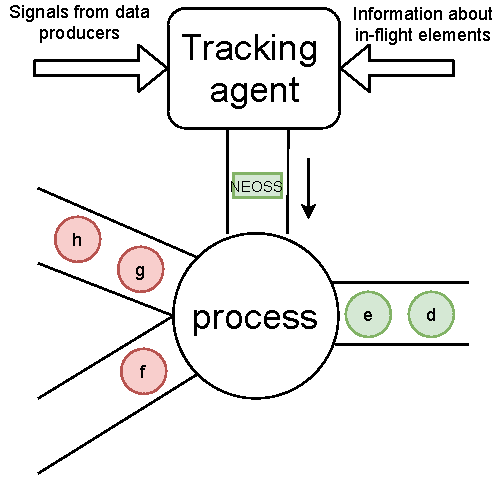
\includegraphics[width=0.30\textwidth]{pics/tracker-scheme.pdf}
  \caption{\tracker\ framework: tracking agent aggregates information about substreams and produces NEOSS}
  \label{tracker_scheme}
\end{figure}

In this work we formalize the substream management problem and show that the network traffic overhead of the punctuations framework is far from the optimal. We also formally define properties of a substream management technique required by various problems such as state snapshotting to ensure that a newly proposed method satisfy them. 

We introduce a new substream management framework called \tracker. Figure~\ref{tracker_scheme} shows the high-level scheme of our method. 
Within this framework, we use a dedicated agent that receives information about substreams from the entire SPE and sends back {\em end-of-substream notifications} (NEOSS). 
NEOSS messages are propagated through this agent without broadcasting between processes, reducing the amount of extra traffic. Such propagation method is suitable for cyclic dataflows because there is no need to forward service traffic through the cycles. A distributed version of the agent allows an SPE to scale.

Basic comparison between the \tracker\ framework and its alternatives is shown in Table~\ref{solutions-overview-table}. Regarding network traffic, $|\Pi|$ is the number of computational nodes and $K$ is the number of substreams. We can outline that the punctuations framework is the only substream management mechanism that supports arbitrary predicates for substreams, so we use it as a baseline approach in the experiments. The commonalities and differences between the \tracker\ framework and alternative solutions are detailed in Section~\ref{fs-acker-related}.

\begin{table}[t]
    \caption{An overview of substream management techniques}
    \label{solutions-overview-table}
    \begin{threeparttable}
        \centering
        \begin{tabular}{|>{\bfseries}c|c|c|c|c|c|} 
          \hline
          Method & \thead{Arbitrary \\ predicates} & Cycles & Traffic  \\ \hline \hline
          Punctuations & + & - & $O(K|\Pi|^2)$ \\ \hline
          MillWheel* & - & N/A & N/A \\ \hline
          Naiad* & - & + & $O(K|\Pi|^2)$ \\ \hline
          Acker & - & + & $O(K|\Pi|)$ \\ \hline
          \tracker\ & + & + & $O(K|\Pi|)$ \\ \hline
        \end{tabular}
        *progress tracker
    \end{threeparttable}
\end{table}

In summary, our contributions are as follows:
\begin{enumerate}
    \item We provide a formal model of substream management. This model allows us to compare the properties of various substream management systems.
    \item We present a novel substream management technique that achieves a lower bound of network traffic overhead.
    \item We demonstrate \tracker\ performance in comparison to a state-of-the-art approach on diverse workloads.
\end{enumerate}

This paper is an extended version of a conference publication~\cite{10.1145/3524860.3539809}. In this paper we address a scalability problem by introduction of a distributed version of the tracking agent and evaluate it on workloads with increased load. We further expand the theoretical properties of punctuation and tracker frameworks and reveal the motivation behind this work in more details.

The rest of the paper is organized as follows: Section~\ref{fs-acker-preliminaries} formalizes the substream management problem and indicates its main properties. In Section~\ref{fs-acker-tracker}, we introduce a general design of the \tracker\ framework and demonstrate the properties of this substream management solution. Section~\ref{fs-acker-impl} summarizes the implementation of \tracker\ for both centralized and distributed setups with optimizations that can reduce the amount of extra traffic. In Section~\ref{fs-experiments}, we show that the proposed technique is scalable and can outperform alternatives employed in state-of-the-art stream processing engines. The relevant prior research is outlined in Section~\ref{fs-acker-related}. Finally, we discuss our conclusions in Section~\ref{fs-acker-conclusion}.